\documentclass[]{latex/ieeeaccess}
\usepackage{cite}
\usepackage{amsmath,amssymb,amsfonts}
\usepackage{array}
\usepackage{algorithmic}
\usepackage{graphicx}
\usepackage{textcomp}
\usepackage{multirow}
\usepackage{wrapfig}
\usepackage{float}
\usepackage{tabularx}
\renewcommand{\arraystretch}{1.3}
\newcolumntype{R}{>{\raggedleft\arraybackslash}X}
\newcolumntype{Y}{>{\centering\arraybackslash}X}

% \def\BibTeX{{\rm B\kern-.05em{\sc i\kern-.025em b}\kern-.08em
%     T\kern-.1667em\lower.7ex\hbox{E}\kern-.125emX}}


\makeatletter
\def\maxwidth{\ifdim\Gin@nat@width>\linewidth\linewidth\else\Gin@nat@width\fi}
\def\maxheight{\ifdim\Gin@nat@height>\textheight\textheight\else\Gin@nat@height\fi}
\makeatother
% Scale images if necessary, so that they will not overflow the page
% margins by default, and it is still possible to overwrite the defaults
% using explicit options in \includegraphics[width, height, ...]{}
\setkeys{Gin}{width=\maxwidth,height=\maxheight,keepaspectratio}

\usepackage[unicode=true]{hyperref}
% 
\hypersetup{
            pdftitle={RMarkdown Template for IEEE Access Articles},
            pdfkeywords={key, words},
            pdfborder={0 0 0},
            breaklinks=true}
% \urlstyle{same}  % don't use monospace font for urls
% url breaks
\usepackage{url}
\makeatletter
\g@addto@macro{\UrlBreaks}{\UrlOrds}
\makeatother

% Pandoc toggle for numbering sections (defaults to be off)
\setcounter{secnumdepth}{5}

% Pandoc syntax highlighting

% Pandoc header

\providecommand{\tightlist}{%
  \setlength{\itemsep}{0pt}\setlength{\parskip}{0pt}}

%% END MY ADDITIONS %%


% \hyphenation{}

%% Inline enumeration
\usepackage[inline]{enumitem}

%% Define variable for Corresponding author
\providecommand\correspondingauthor{}

\begin{document}
\newlength{\xfigwd}
\setlength{\xfigwd}{\columnwidth}

\history{Date of publication xxxx 00, 0000, date of current version xxxx 00, 0000.} % modify
\doi{10.1109/ACCESS.2017.DOI} % modify

\title{RMarkdown Template for IEEE Access Articles}

%% Show list of authors %%
\newcounter{counter1}
\setcounter{counter1}{1}
\author{
\begin{itemize*}[label={}, afterlabel={}, itemjoin={,~}, itemjoin*={, AND~}]
\item{\uppercase{Author One}\authorrefmark{\the\value{counter1}}{, }\uppercase{(Member, IEEE)}}%
\addtocounter{counter1}{1}
\item{\uppercase{Author Two}\authorrefmark{\the\value{counter1}}}%
\addtocounter{counter1}{1}
\item{\uppercase{Author Three}\authorrefmark{\the\value{counter1}}{, }\uppercase{(Fellow, IEEE)}}%
\addtocounter{counter1}{1}
\item{\uppercase{Author Four}\authorrefmark{\the\value{counter1}}}%
\addtocounter{counter1}{1}
\item{\uppercase{Author Five}\authorrefmark{\the\value{counter1}}}%
\addtocounter{counter1}{1}
\end{itemize*}
}

\newcounter{counter2}
\setcounter{counter2}{1}
%% Show address
\address[\the\value{counter2}\addtocounter{counter2}{1}]{School of Electrical and Computer Engineering, University One of City, City, Postcode (e-mail: \href{mailto:author1@email.com}{\nolinkurl{author1@email.com}})}

%% Get corresponding author
%
\renewcommand\correspondingauthor{Corresponding author: Author One (e-mail: \href{mailto:author1@email.com}{\nolinkurl{author1@email.com}}).}
%
%% Show address
\address[\the\value{counter2}\addtocounter{counter2}{1}]{School of Electrical and Computer Engineering, University One of City, City, Postcode (e-mail: \href{mailto:author2@email.com}{\nolinkurl{author2@email.com}})}

%% Get corresponding author
%
%% Show address
\address[\the\value{counter2}\addtocounter{counter2}{1}]{School of Computer Science, National Institute of Science, City, Postcode (e-mail: \href{mailto:autho3@email.com}{\nolinkurl{autho3@email.com}})}

%% Get corresponding author
%
%% Show address
\address[\the\value{counter2}\addtocounter{counter2}{1}]{Department of Research and Development, University of City, City, Postcode (e-mail: \href{mailto:author4@email.com}{\nolinkurl{author4@email.com}})}

%% Get corresponding author
%
%% Show address
\address[\the\value{counter2}\addtocounter{counter2}{1}]{Department of Research and Development, University of City, City, Postcode (e-mail: \href{mailto:author5@email.com}{\nolinkurl{author5@email.com}})}

%% Get corresponding author
%

\tfootnote{This work was supported by the Name Organization of Country under Grant
Number \#\#.}

\markboth
{FirstAuthor \headeretal: RMarkdown Template for IEEE Access Articles} % modify
{FirstAuthor \headeretal: RMarkdown Template for IEEE Access Articles} % modify

\corresp{\correspondingauthor}

\begin{abstract}
The abstract goes here.
\end{abstract}

% keywords
\begin{keywords}
key; words
\end{keywords}

\titlepgskip=-15pt

% make the title area
\maketitle



\hypertarget{introduction}{%
\section{Introduction}\label{introduction}}

\PARstart{T}{his} is an RMarkdown template for working on papers using
the IEEE Access format, based on the \LaTeX  template available for
download at
\url{https://journals.ieeeauthorcenter.ieee.org/create-your-ieee-journal-article/authoring-tools-and-templates/ieee-article-templates/templates-for-ieee-access/}.
This is not a detailed review of the IEEE Access template, nor the
guidelines on how to write papers that comply with the required
formatting and structure of this journal. You can find some details on
how to prepare papers for this journal at
\url{https://www.sharelatex.com/templates/5a761d0d47ce0af37e1c6035/v/0/pdf?inline=true\&name=IEEE\%20Access\%20template}.

Instead, I focused on describing the small changes I added to be able to
generate PDF documents with the corresponding general formatting of this
journal using RMarkdown.

\hypertarget{description}{%
\section{Description}\label{description}}

I have used the RMarkdown template for IEEE Trans articles, included in
the \texttt{rticles} package. The general styling of the document is
provided in the \texttt{ieeeaccess.cls} file, a \LaTeX class file
provided by the journal.

All the files are contained in a R project (RStudio). The file structure
of the project is:

\begin{itemize}
\tightlist
\item
  The \texttt{images} folder contains all the images and figures used to
  produce this paper.
\item
  The \LaTeX templates and classes are stored in the \texttt{latex}
  folder. Bear in mind that the files \texttt{template.tex} and
  \texttt{ieeeaccess.cls} are the ones used to structure the paper in
  the corresponding formatting, so they should not be changed.
\item
  The \texttt{bib} folder contains the bibliography files, including the
  Citation Style file (.csl) to show the references in the corresponding
  format. This file can be found at
  \url{https://paperpile.com/s/ieee-access-citation-style/}.
\end{itemize}

The template uses three images (bullet.png, Logo.png, notaglineLogo.png)
that have been place in the \texttt{images} sub-directory. The
\texttt{ieeeaccess.cls} file has been modified to be able to access
these images in the corresponding folder. This is the only change added
to the orignal class file.

\hypertarget{authors-affiliations-and-footnotes}{%
\subsection{Authors, affiliations and
footnotes}\label{authors-affiliations-and-footnotes}}

First, I adjusted the ``authors'' section, to be able to translate the
info from the YAML into a comma-separated list of authors, in the order
they have been provided. A reference mark for each author is added,
related to the affiliations/institutions and e-mails corresponding to
each author. I also added the key \emph{membership} to be shown in this
section.

Some other changes in the YAML are the key \emph{corresp}, related to
the author to whom proofs of the paper will be sent, and also the key
\emph{footnote} , to contain information regarding the support,
sponsorship and financial aid for the research project.

\hypertarget{biographies}{%
\subsubsection{Biographies}\label{biographies}}

The last section of the paper is destined to the biographies of the
authors. For such purpose, a \texttt{bios.tex} template has been
created. This template will be included after the body and should be
modified to include the actual information of the authors.

\hypertarget{tables-and-images}{%
\subsection{Tables and images}\label{tables-and-images}}

You can create your tables from your own data using any of the available
r packages of your choice (find some at
\url{https://rmarkdown.rstudio.com/lesson-7.html}). Table
\ref{tab:rtable} has been created using \texttt{kable}.

\begin{table}[t]

\caption{\label{tab:rtable}This is a table caption}
\centering
\begin{tabular}{l|r|r|r|r|r|r}
\hline
  & mpg & cyl & disp & hp & drat & wt\\
\hline
Mazda RX4 & 21.0 & 6 & 160 & 110 & 3.90 & 2.620\\
\hline
Mazda RX4 Wag & 21.0 & 6 & 160 & 110 & 3.90 & 2.875\\
\hline
Datsun 710 & 22.8 & 4 & 108 & 93 & 3.85 & 2.320\\
\hline
Hornet 4 Drive & 21.4 & 6 & 258 & 110 & 3.08 & 3.215\\
\hline
Hornet Sportabout & 18.7 & 8 & 360 & 175 & 3.15 & 3.440\\
\hline
Valiant & 18.1 & 6 & 225 & 105 & 2.76 & 3.460\\
\hline
\end{tabular}
\end{table}

There will be conflicts between the \texttt{longtable} environment and
the two-column format of this paper, so I have opted for not using
longtables in any case. Also, I prefer to inlcude my tables using
\LaTeX  directly, so I can have more control over aspects like borders,
column size, cell spacing and alignment, line breaks, ect. That way, I
don't have to edit again the TEX file after the generation.

As for images, you can see a graph generated from r code in Figure
\ref{fig:rplot}.

\begin{figure}

{\centering \includegraphics{article_access_files/figure-latex/rplot-1} 

}

\caption{This is a graph}\label{fig:rplot}
\end{figure}

\begin{figure}
\centering
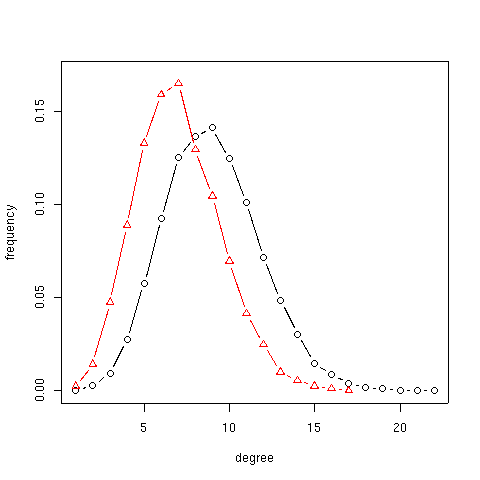
\includegraphics{images/graph.png}
\caption{This is an image\label{fimage}}
\end{figure}

Figure \ref{fimage} shows an image from a file using simple markdown
notation.

\hypertarget{citations}{%
\subsection{Citations}\label{citations}}

The citation style is applied using a csl file, which can be seen
referenced in the YAML.

An in-text for a single author would look like this {[}1{]}. For two
authors, it will be shown like this {[}1{]}, {[}2{]}. Finally, multiple
consecutive references will appear in the following way
{[}1{]}--{[}4{]}.

\hypertarget{recommendations}{%
\section{Recommendations}\label{recommendations}}

When using this template, is important to bear in mind that some
information will have to be modified directly in the TEX file generated
when \emph{knitting} to a PDF (see \texttt{keep\_tex\ =\ true} in YAML).
That will be the case for:

\begin{itemize}
\tightlist
\item
  Date of publication and DOI shown above the title in the first page,
  that can be found as \texttt{\textbackslash{}history\{\}} and
  \texttt{\textbackslash{}doi\{\}} in the .tex file. This information
  would not be available while working on a paper, so it can be left
  blank in the first place.
\item
  Author and title in header, that can be found under
  \texttt{\textbackslash{}markboth} tag in .tex file.
\item
  Volume and year in footer, hard-coded to the .cls file. The have not
  been modified since I tried to keep the changes to the class file to
  the bare-minimum.
\end{itemize}

\hypertarget{references}{%
\section*{References}\label{references}}
\addcontentsline{toc}{section}{References}

\hypertarget{refs}{}
\leavevmode\hypertarget{ref-Dirac1953888}{}%
{[}1{]} P. Dirac, ``The lorentz transformation and absolute time,''
\emph{Physica}, vol. 19, nos. 1 -- 12, pp. 888--896, 1953.

\leavevmode\hypertarget{ref-Feynman1963118}{}%
{[}2{]} R. Feynman and F. Vernon Jr., ``The theory of a general quantum
system interacting with a linear dissipative system,'' \emph{Annals of
Physics}, vol. 24, pp. 118--173, 1963.

\leavevmode\hypertarget{ref-small}{}%
{[}3{]} I. Freely, ``A small paper,'' \emph{The journal of small
papers}, vols. -1, 1997.

\leavevmode\hypertarget{ref-big}{}%
{[}4{]} H. Jass, ``A big paper,'' \emph{The journal of big papers}, vol.
MCMXCVII, 7991.

%% Include authors' biography here

%% Uncomment \clearpage to show authors bio in next page.
%%\clearpage
\begin{IEEEbiography}[{
\includegraphics[width=1in,height=1.25in,clip,keepaspectratio]{images/author1.jpg}}]{Author One} All authors may include 
biographies. Biographies are often not included in conference-related
papers. The first paragraph may contain a place and/or date of birth (list place, then date). Next,
the author's educational background is listed. The degrees should be
listed with type of degree in what field, which institution, city,
state, and country, and year the degree was earned. The author's major
field of study should be lower-cased. 

The second paragraph uses the pronoun of the person (he or she) and not the 
author's last name. It lists military and work experience, including summer 
and fellowship jobs. Job titles are capitalized. The current job must have a 
location; previous positions may be listed 
without one. Information concerning previous publications may be included. 
Try not to list more than three books or published articles. The format for 
listing publishers of a book within the biography is: title of book 
(publisher name, year) similar to a reference. Current and previous research 
interests end the paragraph. The third paragraph begins with the author's 
title and last name (e.g., Dr.\ Smith, Prof.\ Jones, Mr.\ Kajor, Ms.\ Hunter). 
List any memberships in professional societies other than the IEEE. Finally, 
list any awards and work for IEEE committees and publications. If a 
photograph is provided, it should be of good quality, and 
professional-looking. Following are two examples of an author's biography.
\end{IEEEbiography}

\begin{IEEEbiography}[{
\includegraphics[width=1in,height=1.25in,clip,keepaspectratio]{images/author2.jpg}}]{Author Two} was born in Somewhere, City, Country in 
Year. He received a [B.S/M.S.] degree in field from 
the University of Somewhere in Year and other degree, if any.

From Year to Year, he did Some Work as Some Title at Some Place. Since Year, he has been a Job Title at Somewhere. 
He also has done some stuff, like research, authoring books and papers, inventions, and whatnot. 

Author Two was also recognize as Something in Year by Some Institution, and received the Name Award for Something in Year by Some Other Institution.
\end{IEEEbiography}

%% 'ieeeaccess.cls' requires \EOD to indicate the end of the document
\EOD
\end{document}


